%%
%% This is file `sample-manuscript.tex',
%% generated with the docstrip utility.
%%
%% The original source files were:
%%
%% samples.dtx  (with options: `manuscript')
%% 
%% IMPORTANT NOTICE:
%% 
%% For the copyright see the source file.
%% 
%% Any modified versions of this file must be renamed
%% with new filenames distinct from sample-manuscript.tex.
%% 
%% For distribution of the original source see the terms
%% for copying and modification in the file samples.dtx.
%% 
%% This generated file may be distributed as long as the
%% original source files, as listed above, are part of the
%% same distribution. (The sources need not necessarily be
%% in the same archive or directory.)
%%
%% The first command in your LaTeX source must be the \documentclass command.
%%%% Small single column format, used for CIE, CSUR, DTRAP, JACM, JDIQ, JEA, JERIC, JETC, PACMCGIT, TAAS, TACCESS, TACO, TALG, TALLIP (formerly TALIP), TCPS, TDSCI, TEAC, TECS, TELO, THRI, TIIS, TIOT, TISSEC, TIST, TKDD, TMIS, TOCE, TOCHI, TOCL, TOCS, TOCT, TODAES, TODS, TOIS, TOIT, TOMACS, TOMM (formerly TOMCCAP), TOMPECS, TOMS, TOPC, TOPLAS, TOPS, TOS, TOSEM, TOSN, TQC, TRETS, TSAS, TSC, TSLP, TWEB.
% \documentclass[acmsmall]{acmart}

%%%% Large single column format, used for IMWUT, JOCCH, PACMPL, POMACS, TAP, PACMHCI
% \documentclass[acmlarge,screen]{acmart}

%%%% Large double column format, used for TOG
% \documentclass[acmtog, authorversion]{acmart}

%%%% Generic manuscript mode
\documentclass[manuscript,screen,review]{acmart}

%%
%% \BibTeX command to typeset BibTeX logo in the docs
\AtBeginDocument{%
  \providecommand\BibTeX{{%
    \normalfont B\kern-0.5em{\scshape i\kern-0.25em b}\kern-0.8em\TeX}}}

%% Rights management information.  This information is sent to you
%% when you complete the rights form.  These commands have SAMPLE
%% values in them; it is your responsibility as an author to replace
%% the commands and values with those provided to you when you
%% complete the rights form.
\setcopyright{acmcopyright}
\copyrightyear{2018}
\acmYear{2018}
\acmDOI{10.1145/1122445.1122456}

%% These commands are for a PROCEEDINGS abstract or paper.
\acmConference[Woodstock '18]{Woodstock '18: ACM Symposium on Neural
  Gaze Detection}{June 03--05, 2018}{Woodstock, NY}
\acmBooktitle{Woodstock '18: ACM Symposium on Neural Gaze Detection,
  June 03--05, 2018, Woodstock, NY}
\acmPrice{15.00}
\acmISBN{978-1-4503-XXXX-X/18/06}


%%
%% Submission ID.
%% Use this when submitting an article to a sponsored event. You'll
%% receive a unique submission ID from the organizers
%% of the event, and this ID should be used as the parameter to this command.
%%\acmSubmissionID{123-A56-BU3}

%%
%% The majority of ACM publications use numbered citations and
%% references.  The command \citestyle{authoryear} switches to the
%% "author year" style.
%%
%% If you are preparing content for an event
%% sponsored by ACM SIGGRAPH, you must use the "author year" style of
%% citations and references.
%% Uncommenting
%% the next command will enable that style.
%%\citestyle{acmauthoryear}

%%
%% end of the preamble, start of the body of the document source.
\begin{document}

%%
%% The "title" command has an optional parameter,
%% allowing the author to define a "short title" to be used in page headers.
\title{Rapid Communities: Scaffolding the Social Presence in Massive Open Online Courses}

%%
%% The "author" command and its associated commands are used to define
%% the authors and their affiliations.
%% Of note is the shared affiliation of the first two authors, and the
%% "authornote" and "authornotemark" commands
%% used to denote shared contribution to the research.
%\author{}
%\authornote{Both authors contributed equally to this research.}
%\email{trovato@corporation.com}
%\orcid{1234-5678-9012}
%\author{G.K.M. Tobin}
%\authornotemark[1]
%\email{webmaster@marysville-ohio.com}
%\affiliation{%
% \institution{Institute for Clarity in Documentation}
% \streetaddress{P.O. Box 1212}
% \city{Dublin}
% \state{Ohio}
% \postcode{43017-6221}
%}

%\author{Lars Th{\o}rv{\"a}ld}
%\affiliation{%
 % \institution{The Th{\o}rv{\"a}ld Group}
  %\streetaddress{1 Th{\o}rv{\"a}ld Circle}
%  \city{Hekla}
 % \country{Iceland}}
%\email{larst@affiliation.org}

%\author{Valerie B\'eranger}
%\affiliation{%
 % \institution{Inria Paris-Rocquencourt}
%  \city{Rocquencourt}
 % \country{France}
%}

%\author{Aparna Patel}
%\affiliation{%
 %\institution{Rajiv Gandhi University}
% \streetaddress{Rono-Hills}
%\city{Doimukh}
%\state{Arunachal Pradesh}
%\country{India}}

%\author{Huifen Chan}
%\affiliation{%
% \institution{Tsinghua University}
% \streetaddress{30 Shuangqing Rd}
% \city{Haidian Qu}
% \state{Beijing Shi}
% \country{China}}

%\author{Charles Palmer}
%\affiliation{%
% \institution{Palmer Research Laboratories}
% \streetaddress{8600 Datapoint Drive}
% \city{San Antonio}
% \state{Texas}
% \postcode{78229}}
%\email{cpalmer@prl.com}

%\author{John Smith}
%\affiliation{\institution{The Th{\o}rv{\"a}ld Group}}
%\email{jsmith@affiliation.org}

%\author{Julius P. Kumquat}
%\affiliation{\institution{The Kumquat Consortium}}
%\email{jpkumquat@consortium.net}

%%
%% By default, the full list of authors will be used in the page
%% headers. Often, this list is too long, and will overlap
%% other information printed in the page headers. This command allows
%% the author to define a more concise list
%% of authors' names for this purpose.
\renewcommand{\shortauthors}{Trovato and Tobin, et al.}

%%
%% The abstract is a short summary of the work to be presented in the
%% article.
\begin{abstract}
Participants in MOOCs often felt isolated with less peer interactions. MOOC forums often populate with cognitive presence and lacks social presence. Social presence is connecting and interacting humanly using communication. It is an essential component to bring  effective learning experience in any online learning environment. We draw inspirations from \textit{communities of practice} to impend \textit{social presence} in MOOCs and present rapid communities: deliberately created communities scaffold through a process of Cluster, Orient, Focus and Network with infrastructure and tools to cultivate social presence in MOOCs. The rapid communities leverages clustered groups with a community leader facilitating the conversations leading social presence. It provide infrastructure and tools to incubate the social presence and thereby increase the learning experience of the participants. An exploratory case study of integrating rapid communities to a real MOOC was conducted. We present the analysis of unfolding social process under the lens of social presence constructs and communities of practices. Quantitative and qualitative measurements used in analysis with Social Network Analysis (SNA) and Epistemic Network Analysis (ENA). Further, the analysis distinguishes the behaviours of MOOC participants in rapid communities to the general MOOC. Findings of SNA revealed potentials of developing social presence to MOOC by rapid communities and ENA strengthens the findings of SNA by revealing strengths of social presence constructs. The study revealed substantial differences in how learners in rapid communities establish social presence, opposed to the general MOOC as a result of establishing communities of practices. In general, MOOCs are highly populated with cognitive presence, yet the promising social presence in the carefully scaffold communities reflected the feasibility of incubating and scaling social presence in MOOCs. The emergent social processes designed in a scaffold community setting can be a direction which MOOC designers could utilize to open up more opportunities propagate social cues and scale the long missing social presence in MOOCs.

\end{abstract}

%%
%% The code below is generated by the tool at http://dl.acm.org/ccs.cfm.
%% Please copy and paste the code instead of the example below.
%%
\begin{CCSXML}
<ccs2012>
 <concept>
  <concept_id>10010520.10010553.10010562</concept_id>
  <concept_desc>Computer systems organization~Embedded systems</concept_desc>
  <concept_significance>500</concept_significance>
 </concept>
 <concept>
  <concept_id>10010520.10010575.10010755</concept_id>
  <concept_desc>Computer systems organization~Redundancy</concept_desc>
  <concept_significance>300</concept_significance>
 </concept>
 <concept>
  <concept_id>10010520.10010553.10010554</concept_id>
  <concept_desc>Computer systems organization~Robotics</concept_desc>
  <concept_significance>100</concept_significance>
 </concept>
 <concept>
  <concept_id>10003033.10003083.10003095</concept_id>
  <concept_desc>Networks~Network reliability</concept_desc>
  <concept_significance>100</concept_significance>
 </concept>
</ccs2012>
\end{CCSXML}

\ccsdesc[500]{Computer systems organization~Embedded systems}
\ccsdesc[300]{Computer systems organization~Redundancy}
\ccsdesc{Computer systems organization~Robotics}
\ccsdesc[100]{Networks~Network reliability}

%%
%% Keywords. The author(s) should pick words that accurately describe
%% the work being presented. Separate the keywords with commas.
\keywords{datasets, neural networks, gaze detection, text tagging}


%%
%% This command processes the author and affiliation and title
%% information and builds the first part of the formatted document.
\maketitle

\section{Introduction}
Massive Open Online Courses (MOOCs) often face challenges due to their core design --- being open and massive. Openness enables any participant to enroll to any courses at anytime and as a consequence, it is likely that at any given time there is a significant number of students enrolled with fluctuating interactions in courses than at any typical closed online course~\cite{oleksandra2016untangling}. Student interactions in MOOCs are often limited to the space in the forum. However, researchers have repeatedly claimed forums are either disorganized, unused or lead to chaos with massive discourses~\cite{coetzee2014should}. Student interactions are very important for learning, specially the interactions among students which stimulate socialness, enhances psychological motivation to learn~\cite{coetzee2014should}. Researchers claim that for a better learning experience, social interactions are crucial~\cite{yang2007students}. Social interactions bring social presence to a course, yet MOOCs are notoriously labeled as being lacking in social presence and only limited discourse takes place in forums~\cite{antonaci2019gamification}. Furthermore,
learning science and contemporary educational research demonstrates that engagement in peer interactions can bring numerous cognitive and socio-emotional benefits. The notion of belonging to a group and establishing the trust to communicate constitute to a healthy community and the interactions fostered through these communities often reflected as social presence. 

In this paper, we focus on lack of \textit{social presence} as an exemplar challenge that arises in MOOCs where it leads participants in isolation and increase boredom to continue the course. Platforms for learning at scale, especially MOOCs often designed to disseminate knowledge thus learners are less engaged with peers. Limited interactions in forums mostly reflects cognitive presence such as students often tend to ask questions only relating to the course work, assignments, quizzes and errors or help need in platform problems. Therefore, discussions relating to non course work, shared identity, social cues, knowing people, belonging to a group often lacks in the forum. Such social discussions often take place outside of MOOC platforms due to the lack of features supporting such interactions~\cite{veletsianos2015digging}. 


To overcome the challenges arise due to lack of social presence and to scaffold social presence to MOOCs, we draw inspirations from learning concepts: communities of practice (CoP). It describes a social learning theory with a strong relationship to the social construction of knowledge. CoP occurs when groups of people share a common goal or passion for something they do and when they learn how to do it better while interacting regularly \cite{wenger1999communities}. Essentially, CoP contributes to social constructivist model of knowledge where learning occurs in a context of social interactions leading to understanding. Mostly in the online learning, the social process diminish due to its design and conduct.Even for participants, it is culturally challenging to socialise online while building a community. In particular to MOOCs, it is more challenging since the platform is limited to disseminate content and usually the courses does not span for longer period to build strong communities to leverage social presence. MOOC communities with social presence often found in Facebook groups or twitter groups. In previous,  attempts to bring peer interactions to MOOCs had various forms. Such as improving the forum to have a reputation so the discourse enrich with social interactions and interventions such as Talkabout, a online meeting scheduling intervention for social learning~\cite{kulkarni2015talkabout}. However, learning analytic research often examine the social process in MOOCs and highlight the need of contextual sustainable interventions~\cite{poquet2018mooc}. The process of social learning in technology design and innofusions ~\cite{williams2005social} research in CSCW  must explore  challenging landscape of newly emerging phenomenons, such as in this context, MOOC designers constantly disbanding the social process of learning at scale. Epic changes in platform behaviours are needed and desirably a socio-technological solution which impend effective techno-cultural rituals to bring value to the learning experience. 

\begin{figure}[h]
  \centering
  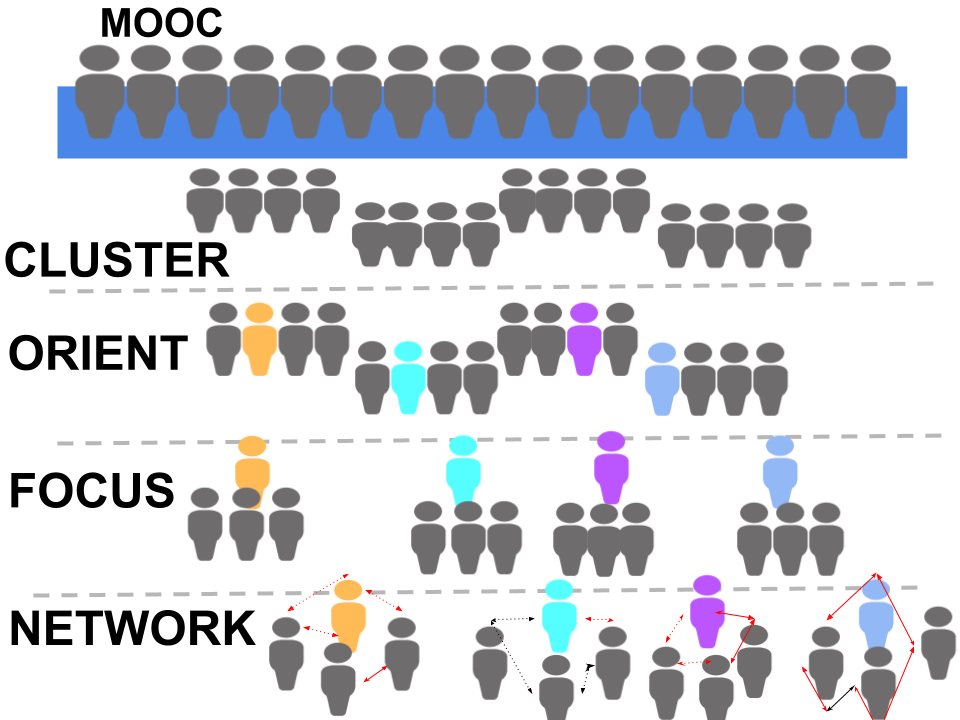
\includegraphics[width=\linewidth]{images/Framework.png}
  \caption{The basic design of the Rapid MOOCs: A regular course with massive participants will be clustered to small communities and provide an orientation with a facilitator, and focus the conversation while networking with peers.}
  \Description{framework}
 \label{fig:framework}
\end{figure}

We present \textit{rapid communities}: deliberately created community space with a scaffold infrastructure and tools incubating social process by Cluster, Orient, Focus and Network. It enabled social presence by \textit{clustering} participants into smaller communities, \textit{orient} the group with a selected facilitator (a member from the group who act as a community leader) with community guidelines, \textit{focusing} the discussions, setting norms and engaging small talk conversations to lead social interactions while stimulating an environment to \textit{network} with the group propagating identity to the community (see Fig.~\ref{fig:framework}). This created an environment of relatively small community with a leader motivated to practise the social process in the community. While rapid communities focus here on impending social presence, our experiment implementation to a real world MOOC explores how rapid communities could address other challenges such as fostering support, collective learning, decision making and social networking with the community peer group (such as,  will the community meet online, will they work collectively and how can work collectively throughout a short time span..etc.), Since the existing platforms does not contain the infrastructure support to design these affordances, we have implemented rapid communities on a German MOOC platform.

The concept of communities of practice introduced in work by Wenger et al~\cite{wenger1999communities} can be applied to any domain, such as any government, organization, social sector, association and to the web as well. All it needs in a communities of practises is a \textit{domain}, a \textit{community} and a \textit{practise}. To focus our exploration, rapid communities designed on a MOOC platform in the domain of web and specifically online learning at scale. Although, CoP as a concept used to enhance effectiveness in any domain, the success of the CoP dependents on design of the structural elements of domain, community and the practice they follow. However, CoP does not provide explicit frame or a dominant model to transform and operationalize CoP in to a community in any domain~\cite{li2009evolution} but a set of principles to affirm the success~\cite{wenger2002seven}. In rapid communities, we articulate a community design with Cluster, Orient and Network while incorporating tools, infrastructure and process to build artificial community rapidly to induce social presence in any course in a MOOC. 

An exploratory case study used to explore the initial feasibility of the integration of the rapid communities. We integrated\textit{rapid communities} to a 6 weeks course (Introduction to Programming in Java) in the MOOC platform where the course had more than 25000 enrollments. We created spaces for rapid communities and in the beginning of the course and then invited any interest participants to take part in the rapid communities as an optional element to the course which has no official credits for taking part or not taking part. Therefore, there were participants who took part in just the main course and participants who took part in the course while in the rapid communities where they were incubated through community space which had cluster, orient, focus and network. We analyzed the social presence in the discourse of the MOOC along with the discourse in rapid communities under the lens of social presence and communities of practices using Social Network Analysis(SNA) and Epistemic Network Analysis(ENA). SNA methods provided an understand of the  frequency  and  intensity  of  co-occurrences  of  dyads in discourse, along with the structure capturing the co-occurrences of social interactions among MOOC participants. ENA aid us to understand the types of conversations and the structural influence of their contributors, which drove the formation of social interactions both quantitatively and qualitatively. Results indicate emerging social gaze situating social presence in the rapid communities than the general discourse of the MOOC while rapid communities demonstrate the ability to make sense of community.  

In sum, participants in MOOC spaces are feeling isolated, lacks peer interactions, affections and group cohesion  and thereby no social presence leading to sense of community. It requires enormous self regulation force to keep them engaged and motivated to learn. Presented rapid communities try address the issues and make following contributes to the CSCW: 

\begin{itemize}
\item \textit{Rapid Communities}, a socio-technical system to integrate social presence in MOOCs and scale by scaffolding the social process by Cluster, Orient, Focus, Network with Infrastructure and tools.  
\item A \textit{exploratory case study} that finds the feasibility of integrating rapid communities to a real live course in MOOC platform. Results suggests the rapid communities are capable of impending social presence to the MOOC while propagating communities of practise which cultivate sense of community.
\end{itemize}

We envision that rapid communities will trigger the value of social learning in MOOCs and act as a re-designed space for MOOC platforms. Not just the social presence, we aspire the rapid communities to be the force to cultivate a learning and knowledge creating atmosphere to MOOCs than participants consuming content. Next, we present details of the concept communities of practice, related work in MOOCs, and introduce our design: rapid communities. Finally, we present the case study with its results and discuss implications of the design.

\section{Background and Related Work}
We first provide a background to Massive Open Online Courses (MOOCs) and its main challenges. Next, overview of the concept of communities of practices and social presence which we incorporated in designing rapid communities. Related prior scholarship on MOOCs community building, social presence and communities of practice were examined. 

\subsection{Background to MOOCs}
Massive Open Online Courses (MOOCs) is an educational technology with a purpose of serving to an open and wider audience. The open nature of it allows any student to join any course and study from anywhere in the world. The concept of MOOCs got attention in 2012 when New York Times called it a "Year of MOOC" ~\cite{pappano2012year}. Mainly because the major platforms for MOOCs such as Coursera, edX and Udacity were introduced during the time. The courses in these platforms are identified as xMOOCs which has a similar structure in every course in their respective platforms such as short videos, quizzes, peer reviews, and forum discussions~\cite{bali2014mooc}. This structure identified as xMOOCs and since its inception, xMOOC model has been criticized in many levels. Mainly its design and pedagogical development of platform and courses. Researchers highlight many issues~\cite{fournier2015mooc,auyeung2015mooc} arising through MOOC research, specifically 7 major issues by ~\cite{scanlon2017learning}, highlight the importance of social learning, optimal group size for learning than massive size, requirement of MOOC success definitions (should not depend on merely pass-rate), types of audience, peer review issues and course credentials. We focus on social learning component which identified as an important research issue in the area of learning at scale.  

Social interactions lead to social learning. Currently the main kind of social interaction supported in MOOCs are online forums; usually threaded discussion of posts and replies, comments visible to all the participants in the course. Forums are imperative in MOOCs to interact and for effective learning experience, but investigations of MOOC forums show struggles to retain users over time~\cite{coetzee2014should} such as half of forum users ceased participation due to factors
such as lack of forum facilitation, an overwhelming number of messages, and rude behavior of other students~\cite{mak2010blogs}. Since forums are disorganized, hard to navigate and develop closer interactions leading to social engagements ~\cite{almatrafi2018systematic}, as an alternative informal groups associated with MOOC courses tend to spring up using social media to create community of learners to bring social aspects of learning~\cite{koutsakas2018exploring}. 

Related word by Coetzee et al~\cite{coetzee2015structuring} attempts to impend the peer learning to MOOC by structuring the peer interactions by a framework where groups of learners are formed on demand and then proceed through a sequence of activities that include synchronous group discussion about learner-generated responses. In that controlled lab experiment authors revealed a structure that required synchronous component and also recommend incentives mechanism for interactions~\cite{coetzee2015structuring}. However, we highlight that MOOCs in nature is different to online learning and field experiments are important to understand the in depth implications of such structuring. Researchers claim that effective forums contribute to enhance student learning's while building community of sense, and collaborative dialogues~\cite{luca2004using}. Although forum contribution frequency has impact on MOOC retention or created a reputation, having higher posting frequency or like buttons with reputation in forum did not support for students to have a sense of community~\cite{coetzee2014should}. In other words, frequent forum engagements which geared reputation did not support the claim for students to have a group sense or belonging to a community, learning with each other.

The notion of sense of belonging found to be an essential item for learning experience in MOOCs and researchers suggest Gamification components to enhance the social presence and thereby impend sense of community~\cite{antonaci2019gamification}. Similarly, early research to understand facilitation through small groups~\cite{lim2014initial}, empirical research work on supportive technologies for group discussion in MOOCs provide substantial evidence of how discussions could redirect to effective learning in collaborative learning environment~\cite{rose2015supportive}. Particularly, Rose et al~\cite{rose2015supportive} case study revealed insights into the limitations of learning through discussion in current xMOOCs, as
well as the challenges in instructor ability to overcome those limitations without support. Community discourse research~\cite{mitchell2011profound,resnick2015socializing} offer convincing evidence for the value of discussion for learning and social engagement but in xMOOCs larger audience of participants never post or reply or identified as likers~\cite{ferguson2015examining,clow2013moocs}. Only smaller potion as regular participants reflect much interactions. Therefore, much empirical understanding into dynamic of structuring, navigating social component's in communities of collaborative learning environments in xMOOCs are needed. One such area toward this goal is leveraging community development and extract social learning for better learning experience in MOOCs. Next we describe such concepts and related work in MOOCs.


\subsection{Communities of Practices}
Our inspiration to build \textit{rapid communities} come from the concept "Communities of Practices" by Wenger et al~\cite{wenger2010communities}. Wenger believe that learning is central to human identity. Humans are social creatures, learn more effectively when they take learning as social participation~\cite{gauvain2007socialization}. With a primary focus on learning as social participation where the individual as an active participant in the practices of social communities, and construction of their identity through these communities were found to be the recent understanding of communities of practice~\cite{wenger2002cultivating}. 

However, in the literature, researchers often used the term "Community of Practice" and "Communities of Practice" to explain behaviours of learning communities interchangeably~\cite{rogers2000communities}. Nonetheless, first developed concept was the "Community of Practice" by anthropologist Jean Lave and educational theorist Etienne Wenger collectively in their book "Situated Learning"~\cite{lave1991situated} which was based on the theory of legitimate peripheral participation. In that concept, they focused more on how community of participants learn things outside the classroom, specially how novice learners learn from experts. Later Wenger focused more towards organizational knowledge structures and defined "Communities of Practice" as \textit{groups of people who share a concern, a set of problems, or a passion about a topic, and who deepen their knowledge and expertise in this area by interacting on an ongoing basis}\cite{wenger2002cultivating}. 

The later concept is more applied to improve organizational performances but generalized to be able to apply to any domain. In the context of learning as a social activity, communities of practice is a group of individuals participating in communal activity, and experiencing and creating their shared identity through engaging in and contributing to the practices of their communities. In order to use CoP as a tool for social learning communities, Wenger  et al ~\cite{wenger2010communities} describe 3 compliance of characteristics: 1) Domain, 2) Community and 3) Practise. Domain creates the common ground (i.e., non member and member status) and outlines the boundaries that enable members to decide what is worth sharing and how to present their ideas. The community creates the social structure that facilitates learning through interactions and relationships with others. The practice is a set of shared repertoires of resources that include documents, ideas, experiences, information, and ways of addressing recurring problems. In essence, the practice is the specific knowledge the community shares, develops, and maintains. Although it is said that all 3 characteristics working together makes effectiveness, it was not explicit on how any one could transform or the level of strengths in combinations of 3 characteristics works better for particular context~\cite{li2009evolution}. 

At the same time, Wenger et al introduce facilitator role to the CoP, where leader or a responsible person who would steer the community and support day to day activities. Although the role of the facilitator was not explicit, many further research were build upon the social structures for communities of practice such as facilitator to be the leader, facilitator and leader to be separate role, facilitator recruitment, merging the role of facilitator and leader etc~\cite{tarmizi2005facilitation}. However, it is important not to be confound on facts that communities of practice are not only self created, but sometimes deliberately cultivated. At the same time myths such as role of facilitator does not arise naturally,  or CoP itself is informal and community build over time,  or think that facilitator role is  always informal, have been debunked by Wenger in their well structured timely maintained official webpage~\cite{Wenger@site}.  


Transforming or creating CoP to virtual is considered for our research. Online CoP often called "Virtual Communities of Practice (VCoP)", understanding the dynamics and how organizations
intentionally form and develop VCoP has been studied~\cite{dube2005impact}. The empirical understanding of the challenges faced in CoP to VCoP examined in 14 organizations which attempted to form 18 VCoPs. The qualitative observations and coding of structural predefined characteristics of these VCoP revealed that success of VCoP is not one dimensional. The observations in VCoP is systemically categorize as demographics,
with overall orientation, life span, age and maturity level of the VCoP, elements of the organizational context in which the VCoP evolves(creation process, level of boundary crossing, environment, membership(size, geographic dispersion, membership stability,
enrollment and selection process, prior community experience, level of ICT literacy), technology (VCoP’s overall degree of reliance on ICT and the variety of ICT available to the VCoP’s members)~\cite{dube2003towards} and examined how co-occurrences of these categories reveal success of VCoP. 

In the context of MOOCs, many research examined CoP (or VCoP since its online) how emergent learning platforms equipped with new technologies are benefiting to informal learning, specially how learner driven communities for professional development~\cite{chae2018enhancing}. Wenger and Lave's early CoP was examined in a MOOC on how alumni and tenured participants support the novice in chat discussion~\cite{nelimarkka2015alumni}. Although such research examined the CoP in the natural MOOC setting, but integrating IRC chat interface in synchronous interactions, they provide valuable insights to design affordances to support the creation of new communities of learners. For communities to practice in a domain, it is essential for learning environments to extend their reach beyond peers and instructors~\cite{bruckman2002future}. Although MOOCs extend their environment for content and peers, communities would not just emerged with the technology, it needs the structuring and cultivation to sustain healthy interactions and engagements. A classic example of such structuring and technology support in CoP described in a case study using OpenHPI MOOC platform~\cite{grunewald2013openhpiF}. Two learning communities observed in the platform under the lens of communities of practice, and provide insights on how platform infrastructure affordances impact the practises. We further extend the insights of it and introduce a structuring process "rapid communities" and systematically impend CoP to reflect social presence.  

\subsection{Social Presence}
Social presence described to the need of users to feel connected with each other and to perceive each other as real people~\cite{gunawardena1997social}. Early researchers linked social presence in communication, medium related phenomena~\cite{short1976social}, then more related to person and social behaviours~\cite{festinger1950social} and later into community with Community of Inquiry (CoI) framework~\cite{garrison2009communities}. Social presence is co-relate to Sense of Community (SoC), the feeling of belonging to a group of members~\cite{liu2009community}. Communities obtain a sense of belongingness through the help of communities of practice (CoP), hence Sense of Community (SoC) and Social Presence are related to Communities of Practice (CoP)~\cite{nistor2015sense} as well. In our research, we try to impend social presence through CoP since social presence is a significant component in enhancing learning experience, specially in online learning, it has found to be critical in improving instructional effectiveness in any setting. With the Social presence, students felt more engaged in their courses. It is a key ingredient for learning yet, many researchers claim that online learning environments often lack Social presence~\cite{kehrwald2008understanding,kim2011investigating}, specially MOOCs~\cite{poquet2018social,kovanovic2018exploring}. 

Social presence in MOOCs have been examined mostly under Community of Inquiry (CoI) framework by Garrison et al~\cite{garrison2009communities} which defines a set of characteristics for investigating online learning as an environment and examine if it is effective. CoI comprises three core elements:“Cognitive Presence”, “Social Presence” and “Teaching Presence”, which interact to facilitate the online learning experience. The framework is based on social constructivist principles with the premise that knowledge is created through interactions with others, that is to say knowledge creation is a social activity~\cite{akyol2009response}. 


Social presence in Garrison's CoI framework defined as "the ability of participants to identify with the community (e.g., course of study), communicate purposefully in a trusting environment, and
develop interpersonal relationships by way of projecting their individual personalities”~\cite{garrison2009communities}. Adopted CoI instrument is extensively used in MOOC context to examine social presence since it is verified, validated and used to proof in many of learning environments. It has 3 main social presence constructs: 1) Interpersonal communication (sometines mentioned as affective communication 2) Open Communication and 3) Group Cohesion or Cohesive Communication. Although some researchers used the survey instrument~\cite{poquet2018social} to examine social presence, forum content analysis and manual coding~\cite{oleksandra2016untangling,joksimovic2015social} for content also practiced in MOOC research. Garrisons Social Presence predictors~\cite{garrison2009communities} are described in the Table ~\ref{tab:Social}, it has been adopted and used by Joksimović et al~\cite{joksimovic2015social} examining social presence relation to academic performance in online courses, where in our research, we used the same model to predict the social presence in the discourse of the communities in the MOOC. 


 

\begin{table}[h!]
\caption{Social Presence Constructs with coded labels and  definitions according to ~\cite{joksimovic2015social} and ~\cite{garrison2009communities}}
 \label{tab:Social}
\begin{center}
    \begin{tabular}{p{3cm}|p{4cm}|p{5cm}}
    % \hline
    \toprule
     \centering Main Social Presence constructs & \centering	Social presence predictors (Label) & Definition  \\
     %\hline \hline
     \midrule
    (1)  Interpersonal communication  &  Affective expression (IE)  & Conventional expressions of emotion, or unconventional expression of emotion, include repetitious punctuations, conspicuous capitalization, emoticons.       
     \\ \hline
      & Self-disclosure (IS) & Presents details of life outside of class, or expresses vulnerability.
    \\ \hline
     & Use of humor (IH)  & Teasing, cajoling, irony, understatements, sarcasm
    \\ \hline
   (2) Open communication & Continuing a thread (OCt) & Using reply feature of software, rather than starting a new thread.
    \\ \hline
     & Quoting from others’ messages (OQ) & Using software features to quote others entire message or cutting and pasting selections of others' messages.
    \\ \hline
     & Referring explicitly to others’ messages (OR) & Direct references to contents of others' posts.
    \\ \hline
     & Asking questions (OA) & Students ask questions of other students or the moderator.
    \\ \hline
     & Complementing, expressing appreciation (OCa) & Complimenting others or contents of others' messages.
    \\ \hline
    & Expressing agreement (OE) & Expressing agreement with others or content of others' messages.
    \\ \hline
    (3) Cohesive communication & Vocatives (CV) & Addressing of referring to participants by name.
    \\ \hline
    & Addresses or refers to the group using inclusive group using inclusive pronouns (CA) & Addresses the group as we, us, our, group.
    \\ \hline
    & Phatics, salutations (CS) & Communication that serves a purely social function; greetings, closures.
    \\ \hline
    \bottomrule
    \end{tabular}
    \end{center}
    \end{table}


%
%\begin{itemize}
%\item \textbf{Affective} construct in social presence is the emotions depicted in the conversations such as Humor, sarcasm, teasing. These are the "Paralanguage" features in text outside formal syntax used to convey emotion (e.g., emoji, punctuation, exclamation, and capitalization). Apart from that, Attempts of Self-Disclosure by describing details of life outside of class, or expresses vulnerability also constitute affects in social presence. We observe these in conversations developing in the forum spaces and report instances.  

%\item \textbf{Cohesive} construct in social presence is the feeling of belonging to a group. Group references and social sharing such as addresses the group as we, us, or our and shares information relating to their work and/or home life. Also the vocatives by addressing or referring to participants by name. We highlight the incurs of these instances in the communities to reflect social presence in rapid communities.

%\item \textbf{Interactive} construct in the social presence in the Interactivity we see between participants. Enagaments with acknowledgement quotes or refers direly to others posts, compliments or agreement in messages, inquiry of questions from other students mostly considered as interactive to social presence and we highlight such occasions in the forum.
%\end{itemize}




\section{Rapid Communities}
Rapid communities are deliberately created community spaces with a scaffold infrastructure incubating social process by Cluster, Orient, Focus and Network. Usually in a MOOCs, thousands of students enroll at any given time. Many MOOC platforms provide a forum space to interact. However, due to the wideness and openness of this space, the discussions tend to overwhelm and is difficult to navigate or have meaningful conversation leading to social interaction.

We considered to transform MOOC to reflect CoP. According to principles of communities of practises~\cite{wenger2002seven}, social capital can be obtained by structuring the community such that it encourage comments, contributions, welcomes newcomers, and regulates behaviour. Wenger et. al defined that CoP draws upon 3 main structural elements: 1) Domain, 2) Community and 3) Practice~\cite{wenger2002cultivating}. Effective CoP can be obtained by leveraging the strengths of these 3 elements. Specifically CoP principles recommend applying wide variety of appropriate leadership sutures, developing community spaces which focus on values while maintaining familiarity and excitement among members~\cite{wenger2002cultivating}. Amid the strong foundations to effective community building, communities of practices lack a strong methodical constructs where anyone can develop, and measure its effectiveness~\cite{li2009evolution}. Therefore transforming MOOCs to a space where it reflect CoP needs structural articulations exclusive to MOOCs. Since CoP itself is evolving and has many interpretations, instead of attempting to bring CoP in specific domain, researchers recommend focusing on optimizing specific characteristics of the concept, such as support for members interacting with each other, sharing knowledge, and building a sense of belonging within networks. Specifically, interventions that facilitate relationship building among members and promote knowledge exchange were eloquent for optimizing the function of these groups~\cite{li2009evolution}. Therefore, based on fundamental challenges in MOOCs and foundation upon 3 elements and such principals in CoP, we explain the rapid communities which scaffolds through Cluster, Orient, Focus, Network and the supporting infrastructure and tools. 

\subsection{Clustering} 
When designing communities of practises for online, previous work relied  on these fundamental characteristics and specifically introduce a phase as "context"~\cite{gunawardena2009theoretical}. It describes the space or environment which create the process of collective intelligence. Wenger et. al defined this as domain, where they set boundaries to distinguish members and non-members~\cite{wenger2010communities}. Following a top-down approach, we create specific spaces in the MOOC where the participants can build their communities and adhere to the practice. Therefore, ~\textit{Clustering} is the process that rapid communities set its boundaries and context. These spaces reflect the boundaries of members and non members. These spaces are residing in the course of the MOOC platform where it divide relatively small number of loosely cohesive participants in the course.  Applying this process to MOOC will create virtual spaces in the MOOC platform which provide an incubator to foster social processes in communities which lead to social presence. We describe more details and the pragmatic process in the exploratory case study. 

\subsection{Orienting} 
Usually a community incorporates a social structure that facilitates learning through interactions and relationships with others ~\cite{wenger2001harvard}. "Practice" in the community is a set of shared experience, knowledge, repertoires of resources that include documents, ideas, experiences, information, and ways of addressing recurring problems~\cite{wenger2001harvard}. In essence, the tacit and explicit knowledge, the cognitive and social interactions we shares, develops, and maintains in community are based on the practice. A practice is not inbuilt to a community or arises it own by creation, it needs deliberate actions to scaffold shared value, engagement, knowledge creation, trust, ownership, collaboration, validation within the community~\cite{liu2009community}. Building community depends on the passion and personal involvement that community leaders bring to their work and the vibrancy of the core group attracted to the centre of the community. 

We re-created the "practice" in CoP to ~\textit{Orienting} in MOOCs by scaffolding a social structure. We introduce a facilitator role with a specific designated name "Community Manager" to each clustered group. The recruitment of the community manager is conducted based on the interest at the course initiation. The role of the Community manager is to facilitate the interactions, keep the community motivated to discussions by social meetings, activities. In this phase participants will be given clear community guidelines to adhere in the community since MOOCs are expected to be populated with diverse participants with varied level of experiences. This also creates a moderating role for the community manager. However, participants also been informed the expectation of the rapid community and how it is different from traditional discussions in the MOOC. The community manager facilitated relatively small group of members make easier to navigate through discussions and develop social process and begin to reflect sense of community. A facilitator may conduct any type of activities in the community where participants feel engaged in socially and cognitively. In order to process smoothly in the orienting phase in rapid communities, it is imperative to comply with certain infrastructure and tools. We describe them later in the paper. Essentially, it is supporting the Community manager to scheduling meetings, fostering and stimulating conversations. In sum, orient in rapid communities defined community manager, community guidelines(a set of guidelines to follow when interacting with other participants), community charter charter:information to the community members of rapid community description and its expectations.



\subsection{Focusing}
To support sustainable growth of the CoP, the commitment of the core members to invest time, effort and participants level of engagement motivation plays a significant role and it makes a community viable and suggests how those activities play out in practice. The principals of cultivating successful communities of practices recommends nurturing a regular rhythm for the community by creating and balancing actions to keep the community engaged~\cite{wenger2002seven}. Keeping the rhythm of the community and meeting expectations entail structuring strategies to focus on sustaining the engagement. Fundamental aspect in the theory of "uses and gratifications" suggests that roiling membership (selecting, recruiting, adding, leaving membership) and continuance use of a virtual community is based on their needs or uses satisfaction or gratification (U \& G)~\cite{sangwan2005virtual}. Implications on understanding sustained membership in virtual community suggest influence of motivational factors on participation is contingent on social learning factors, such as accomplishing online interactions, the complexity of it found found to be positively relating to members to continue in a community~\cite{sun2012understanding}. More specifically, having group norms, social enhancements, commitment and satisfactions of the membership also found to be advocating positively to continue in the community~\cite{cheung2009understanding}. 

Extended such research on MOOCs community development, communities of practice and sustainability in communities were highly underrepresented since at current stage, researchers critically examining  what constitute MOOCs community and its social process~\cite{oleksandra2016untangling,poquet2018social}. Therefore, we lean more towards communities of practices in online learning to draw structural strategies on sustaining the communities of practice. Such research works recommend to implement better communications, establish trust, common values, prior knowledge of membership and sense of belonging , regulating, facilitating, etiquette, user-friendly language, regular interaction, better coordination to achieve regular but varied communication~\cite{bradbury2015role,gannon2007communities}. 

Therefore, we formalize the ~\textit{focusing} in rapid communities by educating community managers to maintain a regular interactions, encouraging multi level participation, keeping the language more simple and social, minimizing the reply latency on post and encouraging more discussion threads. We practically set a culture of addressing each other, socially converse about outside of the class activities such as family life, daytime activities or jobs. 


\subsection{Networking} 
The inter-related concepts of communities of practice, sense of community and social presence entail to build social identity, the notion of knowing a person by their membership from a community or a group~\cite{wenger1999communities}. In Wenger's first model of Community of Practice define "Situated learning theory" which define participation and identity while stating learning is not simply
about developing one's knowledge and practice, it also involves a process of understanding who we are and in which communities of practice we belong and are accepted~\cite{wenger1999communities}.  Individuals in a community develop their identities and practice through participation in a community activities~\cite{handley2006within}. At one level, participation is identified by the action it involved (‘taking part’) as well as
relationships and connections to others in the community. Variations to the degree of participation identified as 1) peripheral where newcomers permitted to participate to a limited extent in simple, relatively discrete tasks and relationships 2) full where key members who participate at the core of the community); and 3) marginal members where participants who are kept at the periphery of the community.   

In relation to MOOCs, such varied level of participation of derived in analysing forums participation~\cite{rodrigues2016discovering,ferguson2012social}. Our goal is to make use of the notion of identity as a factor to impend social presence in MOOCs where within the clusters members building social capital by making friends and bonding behaviors. We coin the participation in CoP to ~\textit{Networking} by providing the stimuli in the focus where the engagement in a small scaled forum space strengthen the social network by ongoing conversations. Therefore articulating ~\textit{Networking} by fostering interactions and relationships based on mutual trust and respect. Such strong learning community fosters interactions and relationships creates a social structure for individuals to share ideas and artefacts (e.g., stories, documents, recordings) that support community activities and help individuals make sense of new knowledge. These conditions provide a rich environment for individuals to share ideas and level the gaps in participation.




\subsection{Infrastructure and Tools}
When designing rapid communities with the essence of communities of practices, the infrastructural arrangements and technological designed tools are imperative for a smooth process of impending social presence.  Articulating process and design of artifacts has a significant impact on the applied social systems. Therefore, the quality of design is not a merely technical infrastructure or feature, but needs to be understood in its interaction with the applying social system~\cite{rohde2009towards}. Attempting to articulate and reproduce a practice needs careful attention, CSCW research stress the importance of in-depth understanding of practices in designing ICT  artifacts~\cite{wulf1995towards} and researchers define a 3 phase research approach such integration, namely \textit{design case study} which includes (1) analyzes empirically the given practices in a specific field of application, (2) comes up with an innovative design for an ICT artifact related to the findings of the first phase, (3) investigates into the appropriation of the technical artifact over a longer period of time. ~\cite{wulf2011engaging}. However, the dynamics of social practices in organizations can be comprehended as interplay between embodied capabilities and dispositions producing  human actions using the artifacts~\cite{wulf1995towards}. Orchestrating these artifacts could incorporate to result objectified operational forms of human actions. Through appropriating the artifacts for effective acting, new incorporated capabilities and dispositions emerge. This enable new ways of behaviours and practices. Studies demonstrate the use of technology and infrastructure to transform communities of practices into knowledge building communities. Specifically provides a framework to scaffold technology into knowledge building community by incorporating tools and techniques to support representation, process and social context~\cite{hoadley2005using}. Incorporating myriad of web tools 


infrastructure required to perform  the community structures,. In order to execute rapid communities, community infrastructure support and tools are required. We execute the rapid communities in MOOCs, therefore MOOC platform should provide the infrastructure to deliberately create community spaces and these spaces must be dedicated to the community incubation without sharing with the General MOOC space interactions. To foster share identities and smooth networking interactions between members  cultivate social identiy and aTools needs to recruit community managers and 



\section{Exploratory Case Study}
In this section we provide pragmatics of integrating rapid communities to the real MOOC. As explained previously, incorporating articulated process of Cluster, Orient, Focus , Network with infrastructure and tools, we conducted the study in the OpenSAP MOOC platform. 

\subsection{Context to the Course in the MOOC}
We selected the course Object-Oriented Programming in Java which spanned for 6 weeks. Creating a course to a MOOC is challenging. Since some of our co-authors were part of the course designing and developing, we had the flexibility to integrate rapid communities to this course. All the authors had ethical clearance and IRB approvals to this research and to handle the pseudonymous data complying with the General Data Protection and Regulation (GDPR). The course was intense with hands-on programming exercises, quizzes, weekly exams, and a final exam. Apart from those, an additional team based assignment was offered to earn bonus points. The course had 27,554 registered participants initially and at the middle only 19,891 participants had continued.  Course offered Record of Achievement (RoA) or Confirmation of Participation (CoP). 2,317 participants (24\%) obtained a Record of Achievement by earning at least 50\% of the available points in the exams and exercises. 3,439 (39\%) of the participants obtained a Confirmation of Participation by accessing at least 50\% of the course material. 


\subsection{Rapid Communities to the MOOC}
In general, all MOOC platforms contain a \textit{discussion forum} that  allows participants and teaching team to interact with each other. Interaction levels may depend on pedagogical and platform designs, yet most commonly courses lack interactivity~\cite{gamage2020moocs}. Rapid communities articulated incorporating MOOC platform OpenSAP. OpenSAP platform is powered by SAP and Hasso Plattner Institute (HPI)~\cite{OpenSAP} in Potsdam and it is structured as a replica of the Hasso Plattner Institute's MOOC platform OpenHPI~\cite{OpenHPI}. OpenSAP more focused to provide SAP's enterprise oriented  courses but similar to OpenHPI, all the courses are open and free of charge. 

Rapid communities need specific infrastructure and tools support to smooth process the Cluster, Orient, Focus and Network. It uses OpenSAP as a vehicle to transform CoP into MOOC. Unlike other MOOC platforms, OpenSAP has specific infrastructure and supporting tools to interact with participants. "CollabSpace" is one of its infrastructure enable to form groups, which are loosely coupled where members can join in and out through the course. In the platform, these groups usually have a self-set goals or a common interest. These groups designed to be self-organized, the participants who creates the CollabSpace has administration privileges and decides if it is public or private (invitation only). Group members can come and go as they want with loosely coupled groups (Anatomy of such infrastructure in this platform explains in more details  ~\cite{staubitz2014supporting,staubitz2017collaboration}). This feature in the CollabSpace enable rapid communities to cluster. 

The process began during the week 0 and week 1 of the live course, Introduction to Java where course instructors sent mails to registered participants informing interested participants to take part in rapid communities, and requesting if any participant would like to lead the community in rapid communities while indicating desire to take part in the community. Using CollabSpace, deliberate spaces were created to incubate social process by the course team based the demand and interest. It is common to see spiked registrations in MOOCs at first where this course had more than 20,000 registrants to the course, but only few percentage continue the course. In this case nearly 2000 participants continue the course while nearly 300 participants were part of rapid communities. In this course, created separate CollabSpaces given some pseudonyms as "JazzyJaguar, LazyLions etc..". However, it is worthy to mention that OpenSAP MOOC platform allowed students to create groups as well, it should not be confuse with rapid communities as those spaces are not scaffolding the social presence by incubating with a process of cluster, orient, focus and network as articulated in rapid communities. Figure~\ref{fig:CollabSpace}, display a screen shot of CollabSpace created these groups for the sake of the study, names of rapid communities were communicated to interested participants and descriptions of the community is displayed in the respective spaces.  

Once students were member of a clustered rapid community, they were given the community guidelines and displayed in discussion board in CollabSpace. In other words, the community orienting and structure is communicated to the participants. Recruitment of the Community leaders were communicated during inquiry of initial interest to take part in rapid communities. Platform generated emails were utilized to inform and communicate the interests. A clear strategical instructions were given to community leaders who display themselves as "Community Manager". Articulating rapid community design required coordination of community leaders and monitoring the progress of the community by the course staff which the platform did not support and tools were required to assist. In this case mostly email communications were utilized. Community Manager given flexibility in responding and directing inquires, stimulating social cues, conducting any meetings with the community or working a problem together with support. Discussion boards (forum space) were utilized for asynchronous communications. This forum space is isolated to the community separating the main discussions take place in the MOOC (See Figure~\ref{fig:CollabSpace}). Once the space is created and assigned a community manager, the community focus the learning from week 1. In this case, they focus on course work, setting norms and rhythm in their communication by synchronous (Google hangout) or asynchronous (Forum posts) mode to discussions, interactions between members while performing actions and proceed through the course in the MOOC. The isolated community space provided effective focusing without been tangled in a larger group of discussions (MOOCs default general discussion forum which all the participants in MOOCs are part of) which bring practical challenges to navigate through work and synchronize together. The separated isolated community brings close knit relationship to the group and sharing identities were more productive and easy leading the social networking and sense of community. CollabSapces provided boundaries to the community where any interest participant can join or leave any time during the course, which made these communities distinguished from teams. By joining, there adhere to the practise imposed in the community facilitated by the community manager. CollabSpace provide tools to effectively interact and network with each other, such as visible profiles, video Hangout, collaborate and share slides, texts and necessary administrative tools to moderate the community space. 

This initial field study allowed us to prototype the rapid communities with minimal development incorporating existing infrastructure and tools in OpenSAP. However, coordination and monitoring needed much effort in this case since we conducted those with emails. Our observations in the integration of rapid communities to MOOCs helped us understand unfolding social process,  capacity to foster interpersonal interactions and challenges to operationalize social organizations. Our objective in rapid communities were to impend long missing social presence in MOOCs and in next section we provide what we observe during these process, how we analysed the outcome. 



\begin{figure}[h]
  \centering
  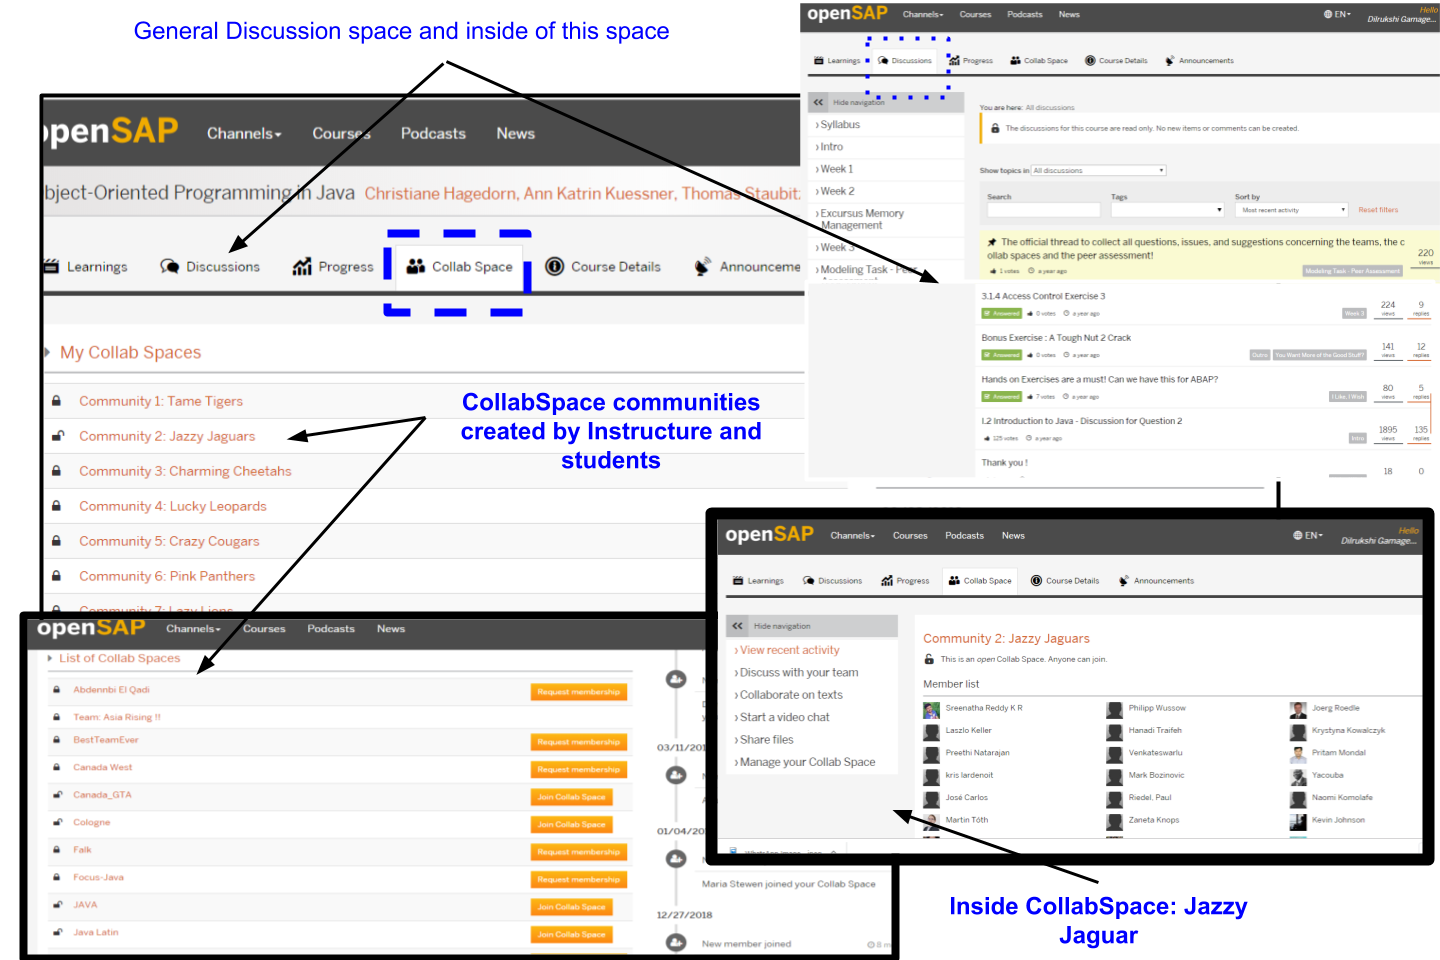
\includegraphics[width=\linewidth]{images/CollabSpacedetails.png}
  \caption{CollabSpace utilized to create rapid communities.}
  \Description{CollabSpace}
 \label{fig:CollabSpace}
\end{figure}



\section{Data Collection and Analysis}
To understand the unfolding social process in the rapid communities, we formulate our analysis towards few populations in the course, a subpulation of rapid communities and the main course. Although the dense of interactions and behaviours are varied in these populations, we considered to analyse the forum activities which commonly supported by the platform infrastructure. Sub population analysis against the main course is conducted in many MOOC analytic research works and recommended due to nature of MOOCs ~\cite{dowell2015modeling, poquet2018socia, joksimovic2015social, oleksandra2016untangling}. At the same time, we made our systematic observations over the course duration to understand the change of behaviours in the cohort and integration experience of communities of practice via rapid communities. Analysis were based on the data gathered in the platform as content and observation notes. Mainly used Social Network Analysis(SNA) methods to understand the interactions and behaviour changes over individuals and content analysis using Epistemic Network Analysis (ENA) method, a Quantitative Ethnographic method commonly used to analyse forum conversations, interactions in learning analytics. The Social Network Analysis (SNA) constructed networks from rapid communities and general course participants in the MOOC. These network structures consolidate the frequency and intensity of co-occurrences of dyads in forum conversations. Apart from SNA, we examined deeply into the content occurred in the rapid communities to understand if its associated with the intended social presence. At the same time conversations of the rapid communities and main cohort were examined against several theoretical constructs relating to learning experience in community  to compare the sociotecho-cultural behaviours using quantitative and qualitative approaches. For this purpose we used Epistemic Network Analysis (ENA).

\subsection{Data}
We gathered the data from the OpenSAP introduction to Java course over a 6 weeks of time. It contained participants lists, forum id, forum content of each participants throughout the course, forum space id, Collabspace id. Also, we obtained the email contents exchanged over the platform regrading information to the course. Apart from these, our own observation data in reflective memos were gathered to enrich the casestudy with experiencing the integration. 

\subsection{Social Network Analysis}
For the purpose of understanding  the participation of online students, it is important to examine their patterns of interaction and their discussions in the forums. Social Network Analysis (SNA) is a valuable tool to examine the dynamics of these discussions: 
\begin{itemize}
    \item It emphasizes the structure and the relationship of the 
actors~\cite{butts2008social}.
    \item It provides insights to the relations and the collaboration patterns of the learners in a forum~\cite{rabbany2014collaborative}.
\end{itemize}
We used the SNA to understand about participants interaction behaviour which is common in learning analytics to identify social capital in MOOCs~\cite{joksimovic2015you}. It visualizes learning engagement in a MOOC and its positive correlation to social network metrics in the discussion forum~\cite{yang2013turn}. Furthermore, it visualizes the social presence of the most active forum users in a course~\cite{oleksandra2016untangling} and help us to find associations between Social Network Position and Social Presence in Communities of Inquiry~\cite{joksimovic2015you,kovanovic2014source}. SNA has been utilized in many studies on MOOCs to untangle the connections in the social capitals of the students~\cite{oleksandra2016untangling,kovanovic2014source} and it has been recognized as one of the most important techniques of social learning analytics~\cite{shum2012social,ferguson2012social}.

We began by constructing a series of undirected weighted networks for rapid communities and general MOOC cohort using Gephi, a software tool for SNA. These networks constituted participants’ co-occurrences in forum discussions. Here the discussions are defined by interactions taking place  while taking turns and engaging in contributing answers to question or socialising. A node reflect a \textit{participant} and edge reflect the \textit{interaction} network construct as if participant\_1 post in the forum and participant\_2 and participant\_3 replied to it, then participant\_1,participant\_2 and participant\_3 would all be linked in undirected edges in a graph. We perform the centrality measures which commonly used to assess the importance of individual nodes to the network. Number of nodes and edges including network density obtained, it indicates the portion of the potential connections in a network to the actual connections. We conduct network measures such as Degree Centrality which gives a measure of a node’s connectivity within a network. This measure useful in recognizing important participants (nodes), as it quickly highlights the nodes with the highest volume of direct connections to other nodes. The degree score was calculated based on the number of direct links a node has to other nodes – incoming, outgoing or both. Similarly we conducted other centrality measures:Betweenness centrality and Closeness centrality which brings most insightful observation on ""who can most efficiently obtain information on other participants in the network or Who could most quickly spread information in a network? Influential participants were identified by the application of k-means clustering to learners’ betweenness and clustering coefficients in both networks.  

%as a way of understanding how important a node is in connecting different parts of the network. Calculated the betweenness centrality score by identifying all of the shortest paths within a network, and then counting how many times a node falls on one. Closeness centrality calculated and  it is similar to betweenness but instead of calculating the number of paths through each node, it calculates a node’s proximity to other nodes. It does this by calculating all of the shortest paths in a network, and then assigning each node a score based on the sum of its shortest paths.

 


\subsection{Epistemic Network Analysis}
Epistemology as a term defines as theory of knowledge and Epistemic Network Analysis (ENA) is identified as a method to operationalize the building of the knowledge. In other words it gives much more operationalization to the behaviours of data to describe complex concepts. Specifically in the direction of learning sciences, epistemic frames will entail to decomposed its complexity into isolated domains such as skills, and knowledge, values, and decision-making which makes it easier to understand the relationships and holistic behavioral differences in complex processes of learning itself~\cite{shaffer2017quantitative}. Epistemic frames will allow to examine complex domains not as set of isolated processes skills, and knowledge, but as a network of
connections among knowledge, skills, values, and decision-making processes~\cite{shaffer2009epistemic,rupp2010evidence}. In this case, the complex process of interchanging and developing social constructs needs to be examined in the MOOC. These social constructs theoretically constitute to \textit{social presence} described in table, yet, to understand these constructs in a temporal discourse in the MOOC need the process of epistemic understanding about social process in a community. Therefore we used ENA to derive and measure the associations of such interlarded complex concepts.

Specifically in the recent MOOCs context, ENA has used by researchers to explore links between social and cognitive presences of communities of inquiry and discover social presence over the time in discourse \cite{rolim2019network}. Specifically this allow the researchers to identify type of interactions in the content which was missed in the SNA method. More relevant to our study,  new framework as SENS approach which is a combination of SNA and ENA method examined on data produced in collaborative activities performed in a MOOC where the researcher suggest that ENA and SNA find complementary and synergistic results \cite{gavsevic2019sens}. 

Contemplating epistemic understanding of behaviours in a new socio-technological design needs careful drilling to unfold the structural understanding of changing and evolving social and cognitive behaviours. ENA was conducted to understand deep connections between complex  social constructs of "Social Presence" develop in the rapid community design. At the same time, we used ENA models to understand the significance between sub populations (main course and rapid community) content occur in forum discussions. The dataset contained the forums posts in rapid communities and general course. To construct ENA, data was coded  against social presence constructs in the Table to reflect the association of social presence in rapid communities. In order to identify any significance in the behaviour, content across the MOOC (rapid community and general MOOC) coded against the Table~\ref{tab:ENAContent}. For each component in a thread (Post, Comment and Message), the coders annotated 1 and 0 for the presence and absence of an indicators of the constructs described in tables.  

\begin{table}[h!]
\caption{The categories of content populated in the MOOC forum}
\label{tab:ENAContent}
\begin{center}
    \begin{tabular}{c|c|p{7cm}}
    % \hline
    \toprule
     Name & ENA code & Description  \\
     %\hline \hline
     \midrule
     Social Task  & S.Task  & Participants’ sense-making of their ability to complete course tasks or understand course content such as grouping,                                        communications          
     \\ \hline
    Socian Non Task  & S.NTask & Non tasks are specially focused on social aspects, i.e. introductions, norm setting or the purpose of MOOCs                    
    \\ \hline
    Cognitive Task  & C.Task  & Conversations explicitly triggered by course tasks, such as quizzes and graded assignments 
    \\ \hline
    Cognitive Non Task & C.NTask & Non tasks were the conversations anything about subject but not in the form of quizzes and questions such as sharing new problems in the subject area 
    \\ \hline
    Administrative Task & Admin & The conversations relating to course administrative problems such as when is the assignment submissions, delay requests 
    \\ \hline
    Error Reporting & Error & Error  reporting in the site or course , software modules   
    \bottomrule
    \end{tabular}
    \end{center}
    \end{table}



\subsection{Observations}
Although our main objective was to examine the impended social presence in MOOCs by integrating a rapid communities, our examinations considered the communities of practise populated through rapid communities. Integrating rapid communities needed effort to carefully structure in a live MOOC. Specifically, the smooth transitions of the phases of Clustering, Orienting, Focus  and Networking. Usage of tools and infrastructure were observed over the course. The "Community Manager" role is a key component in the rapid community, we specifically monitor the exchanges, challenges and behaviours through out the time periods. First auhtor of this paper dedicated to take notes of observations, the changing behaviours and actions by enrolling to the platform. Therefore 0 to 6 weeks of observations in developing conversations analysed. We explored how rapid communities could address challenges such as  fostering support, collective learning and decision making ( e.g., will the community meet online, will they work collectively and how can work collectively throughout a short time span), social networking with the community peer group while debriefing challenges and success of communities of practice endured over the course. 

\section{Findings from the study}

\subsection{Rapid Communities manifest theoretical constructs of Social Presence in MOOC}
We assessed the \textit{social presence} developing in the rapid communities by analysing the content. Our results found significant level of associations between social presence predictors in the rapid communities. We initially coded 3 main social presence predictors against binary indicators by occurrence in the forum data. Forum data has threads which contain levels: a post, a reply and message to a reply, each level considered as unit to compare against the codes. However, we realized the 3 predictors against each thread less support to explain how evolving discussions lead to social presence due to many of the thread contain all 3 main social predictors and it can be better distinguish using a model 0f 12 predictors (which distinguish 3 predictors described in Table). We used 2 coders and they achieved a level of agreement for both presences reaching a (percentage of agreement = 79\%, Cohen's k = 0.786). In the ENA, first we defined the units of analysis in the rapid communities subsetted by threads which has posts, replies and messeges to replies identified by line ID. The ENA algorithm uses a moving window to construct a network model for each line in the data, showing how codes in the current line are connected to codes that occur within the recent temporal context~\cite{siebert2017search} defined as one line complementing each line, plus the previous line within a given conversation. The resulting networks are aggregated for all lines for each unit of analysis in the model. This model aggregated networks using a binary summation where the networks for a given line reflect the presence or absence of the co-occurrence of each codes defined previously (see Table ).(See  Shaffer et al.~\cite{shaffer2016tutorial},for a more detailed explanation of the mathematics and Arastoopour et al.~\cite{arastoopour2015epistemic}, Sullivan et al.~\cite{sullivan2018using} for detail examples of this kind of analysis). Essentially, the model generated by this co-registration of network graphs represents  the associations and its strength of the social predictors. First, we perform the ENA with 12 predictors, but 12 codes model was more complex to provide a meaningful interpretation among 12 predictors. Therefore, we present a ENA model with 3 predictors where the model of social presence predictors in rapid communities had a correlations of 0.97 (Pearson) and 0.96 (Spearman) indicating a strong goodness of model. The model represent strong associations of the social presence constructs where the thick lines found highest strengths in association. The strengths of Interpersonal Communications-Cohesive Communication has the strongest association (3.45) in the model compared to Interpersonal Communications-Open Communication (1.80) and Cohesive Communication-Open Communication (2.10). This can be interpreted as the rapid communities much reflect the Interpersonal and Cohesive communication type conversations such as the conversations about life outside the classroom, emotional experiences, sarcasm, greetings, addressing with in a group mindset. Therefore, with the model fit data and strengths, we revealed social presence in the rapid community. 
\begin{figure}[h]
  \centering
  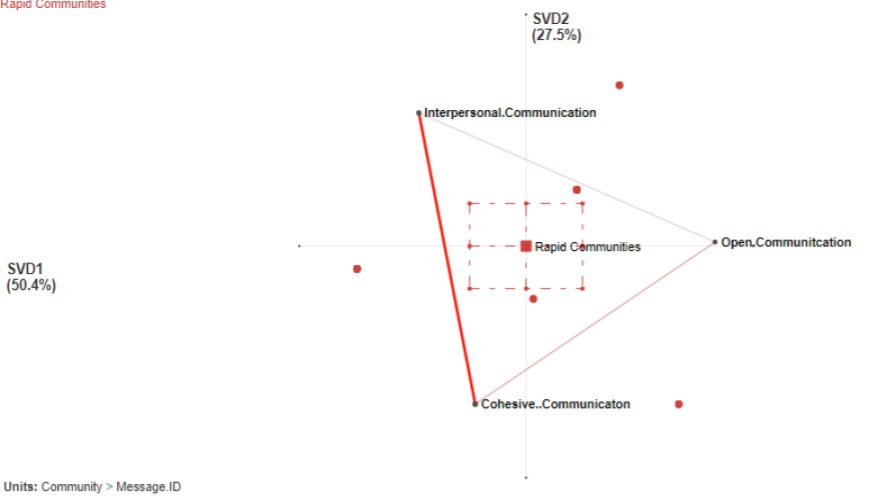
\includegraphics[width=\linewidth]{images/ENASocialP.png}
  \caption{The ENA Model generated using 3 social predictors: Interpersonal, Cohesive and Open Communication. The highest  strengths was from the association of Interpersonal Communications-Cohesive Communication (3.45). Next were Cohesive Communication-Open Communication (2.10) and Interpersonal Communications-Open Communication (1.80).   }
  \Description{framework}
 \label{fig:primary}
\end{figure}

Other than the ENA model from 3 predictors, we also performed a binary factor analysis using the statistical tool R with ‘polycor’ package across the observed content coded with details in 12 predictors (Table ~\ref{tab:ENAContent}) into 3 factors and using verimax rotation. This is mainly to understand the if the observed conversations co-relate to the 3 predictors of social presence and successfully constitute to social presence developed in rapid community. Factor analysis loaded 12 items positively for all 3 factors and sum of squares loadings indicate highest factor loading's for Cohesive communication and Interpersonal communications while moderately loaded on Open Communication. The Table ~\ref{tab:FA} reflect these sum of square loading with variance to the model. This is in other words provide us the evidence of the important items in the social presence predictors which developed in the rapid communities. Cumulative variance of 79.1\% of the 3 predictors determined the social presence to the rapid community. 

\begin{table}[h!]
\caption{Factor Analysis: Sum of Square and Variance of the 3 factors }
\label{tab:FA}
\centering
    \begin{tabular}{c|c|c|c}
    % \hline
    \toprule
     & Cohesive Communication & Interpersonal Communication & Open Communication  \\
     %\hline \hline
     \midrule
     SS loadings &  2.101 &  1.832 &  1.377 \\
    Proportion Var &  0.317 &  0.267  &  0.207 \\
    Cumulative Var &  0.317 &  0.584  & 0.791 \\
    %\hline
    \bottomrule
    \end{tabular}
    \end{table}



\subsection{Differences in Participants interactions in a rapid community and General Course}

Previously we described how social presence is appearing in rapid communities. Next, we try to understand and compare the interactions based on the information exchange in the forum posts. As explained section 5.2, we constructed 2 SNA diagram (See Fig~\ref{fig:SNA} for rapid communities and general course discussion interactions. Both networks were compared to understand the differences using centrality measures.   

\begin{figure}[h]
  \centering
  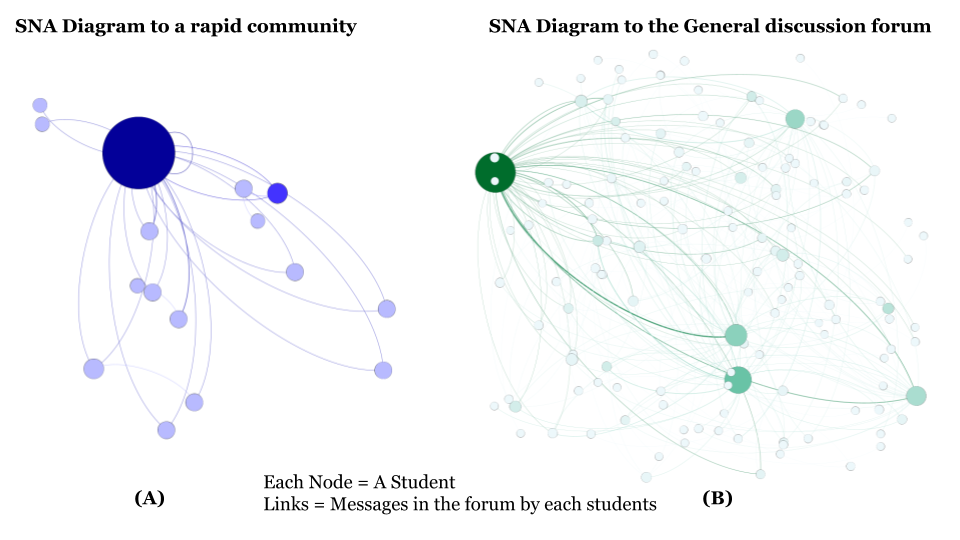
\includegraphics[width=\linewidth]{images/SNA Diagrams.png}
  \caption{Two SNA diagrams constricted using Gephi. (A) for interactions in Rapid communities,(B) the General course discussion.  A node reflect a \textit{participant} and edge reflect the \textit{interaction} where the network construct as if participant\_1 post in the forum and participant\_2 and participant\_3 replied to it, then participant\_1,participant\_2 and participant\_3 would all be linked in undirected edges in a graph.}
  \Description{framework}
 \label{fig:SNA}
\end{figure}


The results suggest that participants in the rapid communities had a higher potential for establishing relationships within its dyads. As depicted values in the Table ~\ref{tab:SNATab}, and Figure ~\ref{fig:SNA}, the structure of co-occurrences for the rapid communities forum contributors was not dense, yet participants co-occurred more often, compared to the general forum. The way we interpret the forum posts, replies, messages may reflect that each participant is interacting with each other and exchanges their ideas in repeated and quick turn taking. Specifically, we could observe the interaction pattern in the rapid communities participants network was structurally dependent on a non-clique of individuals but exchange patterns centered through a key participants which is community leader in this case (see Figure~\ref{fig:SNA})- (A). Due to their brokering power (high betweenness and low clustering coefficient) these individuals brokered information between other contributors. In the General forum network structure, we found several key members in the community constantly replying to others and helping other students in answering questions. They have higher degree centrality and about 4-5 actively contributors were observed (see Figure~\ref{fig:SNA})- (B). Network density reflect the measure of how many interactions between participants exist compared to how many interaction are possible. In this case our networks has different number of nodes to compare both, but proportionally rapid communities reflect slightly higher dense of activities. However, keeping a network density provide a connected group, where in General forum, many of the participants are one time posters and continuing connection is limited. Since such type of frequent contributions of post to the forum does not reflect the social presence in a MOOC, we further analyzed the content of the discussions. 

\begin{table}[h!]
\caption{The Social Network Analysis metrics derived from General forum network and CollabSpace:Jazzy Jaguar}
\label{tab:SNATab}
    \begin{tabular}{c|c|c}
    % \hline
    \toprule
     & General Forum Network  & Rapid Communities   \\
     %\hline \hline
     \midrule
     Nodes	& 2458 & 137    \\
     Edges & 14329 & 456   \\
     Density & 0.02 & 0.038  \\
     Degree & 0.14 & 0.06   \\ 
    Betweennes & 0.183 & 0.212 \\ 
    Closeness & 0.183 & 0.212  \\
    Clustering 
    Coefficient's & 0.107 & 0.08 \\
    %\hline
    \bottomrule
    \end{tabular}
    \end{table}


\subsection{Significant behaviours in content of rapid communities and general MOOC}

The SNA analysis did not demonstrate much of the diference of interactions since posting behaviour is very active in both general course forum and rapid communities. Therefore , we examine content exchanged between the 2 populations. We try to understand the behaviours of the content across the course and rapid communities while identifying any significance. Previous researches often claim that forum discussions are populated with cognitive presence which can be identified as discussions relating to asking questions about the course work, assignments or questions based on the course content or even platform errors. This reflects that forums were mostly demonstrating cognitive type of behaviours. Similar to the analysis conducted by Oleksandra and Shane~\cite{oleksandra2016untangling} to understand the forum behaviours, we categorized the forum content in to qualitative codes. We Incorporated  Oleksandra and Shane~\cite{oleksandra2016untangling}'s qualitative categories to examine forum behaviours. Those are depicted in the Table, additionally based on the emerged category we added error reporting as a new category. However, instead of bipartite network we constructed an ENA network which aid us to understand significant content variations along with the conversations considering temporal phases where the conversations taking place over the weeks. 

\begin{figure}[h]
  \centering
  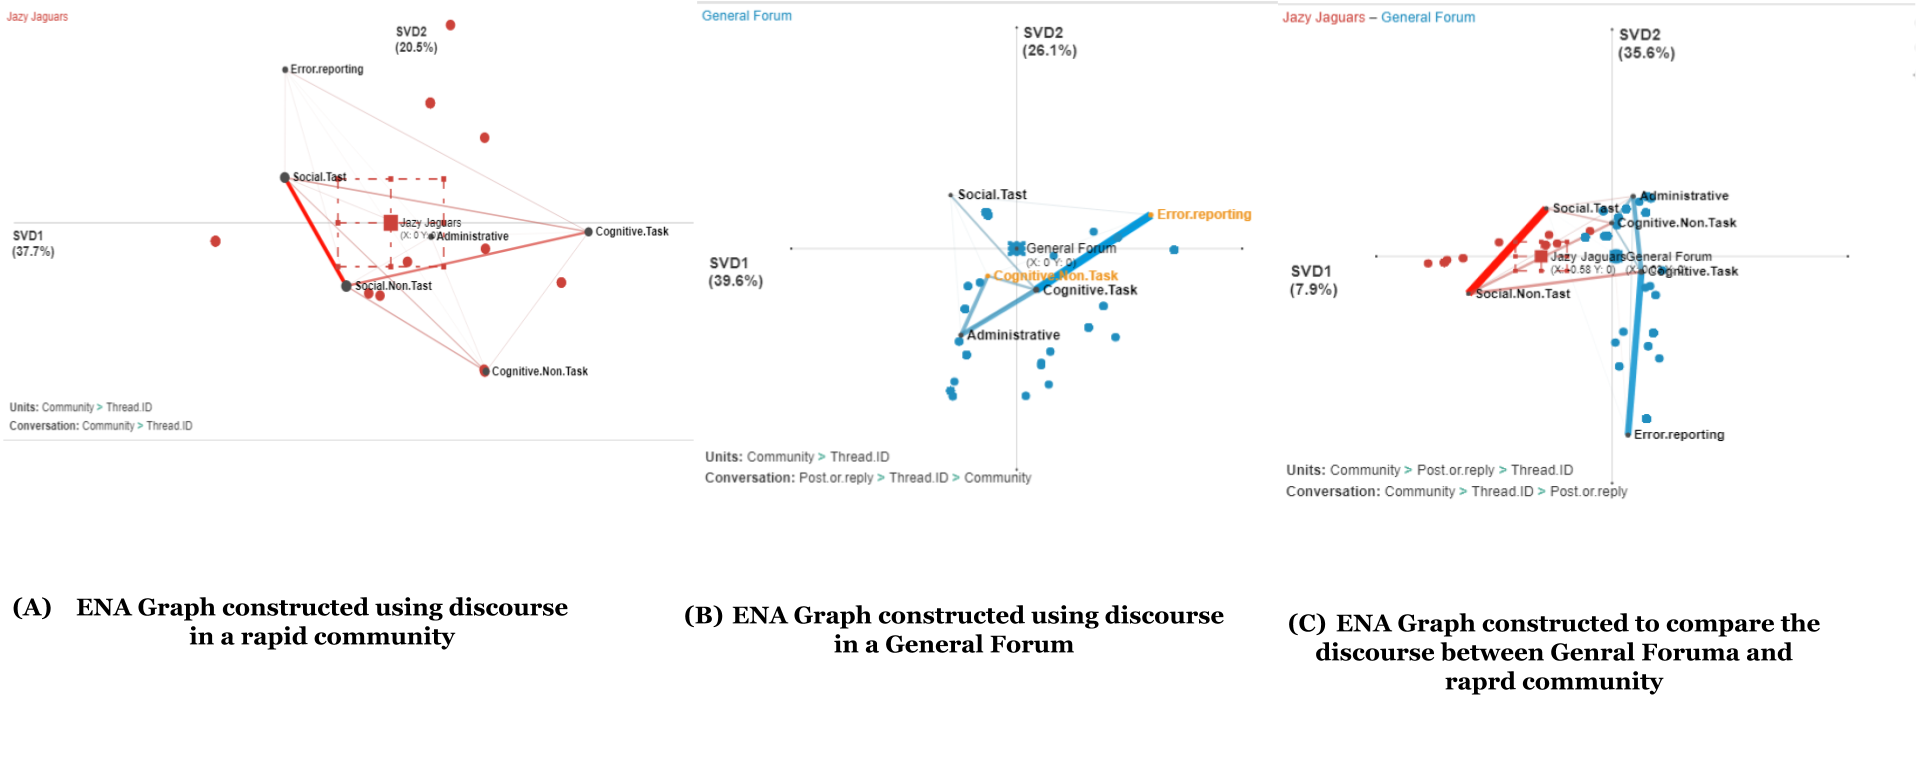
\includegraphics[width=\linewidth]{images/ENA Diagrams.png}
  \caption{The basic design of the Rapid MOOCs: A regular course with massive participants will be clustered to small communities and provide an orientation with a facilitator, and focus the conversation while networking with peers.}
  \Description{framework}
 \label{fig:ENADiagrams}
\end{figure}

In this, we extracted forum data sets from forums in the 1) rapid communities and 2) general discussion in the MOOC and coded using 2 coders according to the code themes described in the Table~\ref{tab:ENAContent}. Three ENA models were constricted forum data by making any level (post, reply, message) of content from forum as unit of analysis.

Model 1 contained the rapid communities, model 2 with main course discussion content and model 3 as a comparison model to distinguish the difference in conversation behaviours.  Figure~\ref{fig:ENADiagrams}- (A), (B), (C) presents the strength of each connections all 3 diagrams with higher values with stronger connections in thicker edges. 

Model 1, Figure~\ref{fig:ENADiagrams}- (A) revealed that, in the rapid communities, there were several strong connections within the social presence indicators, such as the link between Social and Non Social task (2.85) and Social Non Task and Cognitive Task (1.65). It proves the social presence in rapid communities where discussions were more towards sense making, grouping, setting norms and continuing discussions on course along with other relating questions. Therefore we highlight in rapid communities to have i) Strong connection in Social Tasks and Non Social Tasks ii) Non Social Tasks and Cognitive Tasks made to second strong association. iii) There were significant less association between  Administrative conversations and Error reporting in the community. 

Model 2, Figure~\ref{fig:ENADiagrams}- (B) constructed from General discussion of the MOOC presents the higher strengths in Cognitive Tasks and Error reporting (7.5), Cognitive Task and Administrative (4.39), Cognitive Non Task and Administrative (3.46) Cognitive Task and Cognitive Non Task (2.23), Social Task and Cognitive task (1.74). Therefore we highlight that  i) The main forum of MOOC was mostly focusing on subject related direct discussions and also particular to reporting problems of certain java codes not compiling, code errors in the java program in the MOOC. ii) At the same time they made many effort to converse about course administrations issues, such as deadline changes, certificate requirements, questions relating the record of achievements, pass marks etc. iii) Few conversations with regard to questions unrelenting to the java course but general java programming issues were discussed but significant less proportion of conversations made any sense making, grouping of reflected community behaviour. 


Model 3, Figure~\ref{fig:ENADiagrams}- (C) generated as a subtraction model using both model 1 and model 2 to compare the significance's in these conversation type behaviours. This time the model was loaded with forum codes in both communities and ran a non parametric test. Resulted model had a strong goodness of fit with 0.97 (Pearson) and 0.94 (Spearman) co-relation. A non parametric Mann-Whitney test showed that rapid communities (Mdn=-0.45, N=135) was statistically significantly different at the alpha=0.05 level from General Forum (Mdn=-0.04, N=611 U=3947.00, p=0.00, r=0.63). This indicates the conversation behaviours stimulated in the artificially created CollabSpace is significant to general forum. As the resulted model in Figure~\ref{fig:ENADiagrams}-(C), indicates the red thick lines in social parameters were highlighted in rapid communities and in General forum, error reporting, administrative and highly cognitive discussions were remained as highlighted in blue line.





\section{Discussion}
\subsection{Key findings}
Through our exploratory case study of integrating rapid communities to a real MOOC, we learned how structured learning communities with scaffolding can bring desired social components to the MOOCs. Through our rapid communities, we discovered that creating designated spaces with a designated leader entail communities of practice enabling sustained process of social presence.  In this section, we generalize our findings by discussing design implications for future social computing systems and proposing a design space for  MOOCs by using rapid communities as a tool to impose long missing social leaning affordance by cultivating communities of practice. 

\subsection{Implications of Rapid Communities to learning at scale}


\textit{Impose social presence at scale} 

\textit{Articulating community values in MOOCs} 

\textit{Distributed learners to connected learners} 

The involvement of a facilitator is a major component in the scaffolding process and perhaps one of the most frequently observed features in the subsequent studies of CoPs, some of which link the success or failure of the group to this role[7, 13, 35, 46–53].  However, the actual responsibilities and the organizational support provided for this role vary across studies. For example, some facilitators play a distinct role from that of the leader and conduct their activities under the direction of the group and/or the leader[13, 46, 52], while other groups merge the role of the leader and facilitator[47, 48]. The choice of management structure appears to depend on the size of the group and the availability of human resources. Which model best suits which type of organisation is unclear, but facilitator fatigue has been mentioned as something that can lead to the breakdown of CoP groups[47].

In rapid communities, orienting imposed a structure centered through a facilitator to the created community. By means, a recruited member of the community act as a facilitator with a role of "community manager" and all the members in the community space adhere to a community guidelines. 

\subsection{Limitations of the Study}
It is important that we state the limitations in this study for further extensions and reproducability.  
\subsubsection{Selection bias towards platform and course} 
We selected a programming course to our convenience in integrating rapid communities. As a  beginning understand social process in real MOOC setup, selection of programming course may  have impacted as audience may naturally do not expect social interactions but content on programming than a subjective field where it need much discussions such as Introduction to Philosophy. At the same time, our selection of the MOOC platform which had infrastructure inbuilt to the platform where participants are familiar to a culture of  socializing than any other xMOOC platform. However, for that our analysis in the discourse of main course provide a distinct behaviours and significance in content. At the same time, we admit that this is one case study and we are compel to generalise our findings based on more rounds of rapid communities over diverse subjects and more iterations of courses. 

\subsubsection{Sub-populations and Community spaces in the analysis}
As we mentioned, CollabSpace in our MOOC platform allow any participant to create their own spaces which could utilize for learning as a loosely cohesive group. This course also had many such student generated spaces, although we did not directly analyse interactions in those places, it is often less engaged besides it act as a feature with out articulated process of rapid communities. 
In previous research work on MOOCs, forum discussions were recommended to analyse against the sub-population than the entire cohort discussion as a data plane~\cite{poquet2018social}. In this research we derived sub-population from the rapid communities but did not break the main forum discourse into sub-populations. At the same time, participants from rapid communities were not restricted as a controlled group, they were allowed to take part in the main course discussions as well. However, as we did the manual coding of the discourse we did not find a considerable mix or the impact is  limited and neglected since our objective is to impend social presence through rapid communities which has articulated process of integrating CoP. At the same time, we initially created 7 spaces for rapid communities, yet due to limited time and resources, we concentrated on one space with the pseudonym: Jazzy Jaguar and analysis were based on this sub population to the entire course population. 

\subsubsection{Measuring social presence and articulating CoP}
Rapid communities is a articulation process of integrating CoP to the MOOC. Amid there there is no operational method to integrate CoP to any situation, Rapid communities: cluster, orient, focus, network with infrastructure and tool may not the only plausible articulation to integrate CoP to MOOC. Our intention was to impend social presence in MOOCs and rapid communities was the vehicle to achieve the desired goal. At the same time, our measurement to assess social presence were derived from part of previous validate framework: 3 constrcuts of Social presence in Community of Inquiry (CoI) framework, Many learning analytic literature downgrade the CoI model of social presence to MOOCs as CoI model has been developed targeting regular online courses but not not MOOCs and MOOCs posses significantly different behaviours to a regular online course~\cite{poquet2018mooc}.

\section{Conclusions and Future work}
Primary takeaway of our case study is 2 folds. First, we presented an articulation process of integrating communities of practices (coP) to MOOC by introducing \textit{rapid communities}. Our key objective was to bring long missing \textit{social presence} to the MOOC and we demonstrated how communities of practices are linked to social presence. next, we provide a case study of integrating the rapid communities to a real MOOC. Analysis of case study revealed the 1) possessed social presence in the rapid communities, 2) the significance of the conversations as interaction and content across the main mooc and the rapid communities. Main discussion board in the course had high propensity towards association of cognitive type content and Error reporting while rapid communities propensity towards social tasks and non social tasks. Our observations through this integration revealed the challenges building communities in MOOC. 

In future, we plan to enhance the process with more iterations and building new tools and improving the infrastructure to optimize the process(establishing communities of practices) and outcome (social presence). In doing so, some of the the key challenges we face include dashboards to review progress or the success of community spaces, optimizing the community manager requirement process and establishing incentive mechanism to sustain the interactions. Our articulation process of rapid communities is adoptable to any MOOC. Through our socio-techical system we envision a cultural change in MOOC behaviour of content consumers to social learning and knowledge creators. 

.  










%%The community is a group of people who learn and interact together, building relationships that result in a feeling of belonging and mutual commitment~\cite{wenger2010communities}
%==================================
%Learning theories help the designers of learning environments understand what they are fostering. No matter which learning theory the designer ascribes to, communities can provide opportunities for learning. For instance, consistent with the behaviorist tradition, interaction with others in a community can be the feedback that conditions responses to stimuli. Likewise, in the developmental tradition, interaction with peers and nearpeers in a community may provide developmentally appropriate scaffolding.  Clearly, communities provide fertile ground for sociocultural appropriation (adopting expert practices through social processes) as well. In sum, communities could be a venue for learning regardless of the learning theory to which the designer ascribes.

%Wenger In the design of communities of practice, many researchers describe frameworks and guidelines to create communities of practise. to cr the rapid communities Building communities of practices brings participants into a narrow space so they can gain visibility and build meaningful connections. We cluster MOOC learners into groups with a small number of participants with forum spaces for each group. We propose randomised or interest based grouping, however there remains limited consensus on the best grouping mechanism.each cluster then occurs within the forum platform to keep the participants engaged. Each cluster is welcomed by a selected community leader and facilitator. Leaders could be selected in a variety of way such as through prior experience or evaluation. The simplest, and the one we use in this study, is through selecting volunteers from the main participant pool who also have enough time to contribute in this capacity. 


%% The acknowledgments section is defined using the "acks" environment
%% (and NOT an unnumbered section). This ensures the proper
%% identification of the section in the article metadata, and the
%% consistent spelling of the heading.
\begin{acks}
Anonymous during peer review
\end{acks}

%%
%% The next two lines define the bibliography style to be used, and
%% the bibliography file.
\bibliographystyle{ACM-Reference-Format}
\bibliography{sample-base}

%%
%% If your work has an appendix, this is the place to put it.

\end{document}
\endinput
%%
%% End of file `sample-manuscript.tex'.
